\documentclass[12pt]{article}
\usepackage[utf8]{inputenc}
\usepackage{graphicx}

\title{Digital Image Processing \\ Assignment 1 \\ Group No.4}
\author{Abinash Acharya (11840050) \\ Ashutosh Garg (11840250) \\ Thummala Milind Kesar (11841160)}
\date{September 2021}

\begin{document}

\maketitle

\section{Q1 Digital Paths} 
The program files corresponding to Q1 are q1.py and q1\_test.py. \\
q1.py contains the main function paths\_info() \\ 
q1\_test.py is a test script which calls this function with the example inputs provided in Q1. \\ \\
\textbf{Note :- The top-left corner of the 2-D image is considered as the origin to index the pixels. Also, zero-indexing has been used here.} \\ \\
The description of the main function used is as follows : \\ 
paths\_info(I,x1,y1,x2,y2,V,path\_type) \\
The various parameters are defined below : \\ \\
(i) (x\_1,y\_1) :- These are respectively the x-coordinate (row-number of pixel) and y-coordinate (column-number of pixel) of source point. \\
(ii) (x\_2,y\_2) :- These are respectively the x-coordinate (row-number of pixel) and y-coordinate (column-number of pixel) of destination point. \\
(iii) I :- This is a 2-D matrix specifying the intensity values of the image. 
(iv) V :- List of pixel values forming the foreground. \\
(v) Path\_type :- This specifies type of path to be found. It can be 4 for 4-path, 8 for 8-path and 10 for m-path. \\ \\
The steps involved in the process are : \\
(i) Binarizing the matrix using the list V. \\ \\
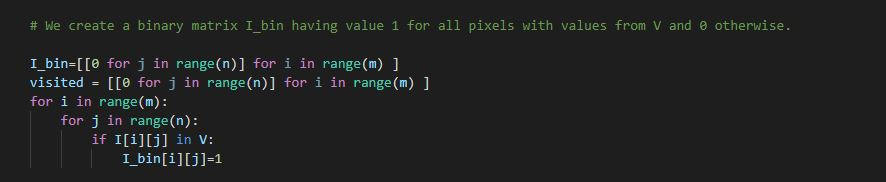
\includegraphics[width=\linewidth]{Binarise.JPG}
(ii) Now, depending on the path type we call the appropriate custom DFS (Depth First Search) function. \\ \\
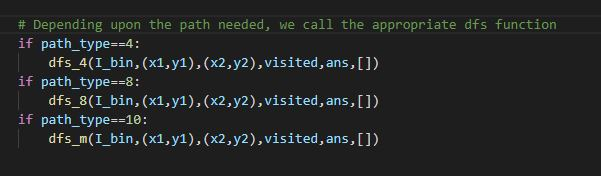
\includegraphics[width=\linewidth]{DFS.JPG} \\ \\
(iii) There are 3 DFS functions, namely, dfs\_4, dfs\_8 and dfs\_m, for 4-paths, 8-paths and m-paths respectively. \\
All of these functions recursively call themselves on adjacent pixels until the destination pixel is reached and the paths obtained (as lists of tuples i.e. coordinates) are appended to the variable 'ans'.\\
(iv) The function paths\_info returns a 3-tuple containing ans (List of paths), Lengths (their respective lengths) and shortest\_paths(List of shortest length paths). \\
(v) Sample image and its output. \\ \\
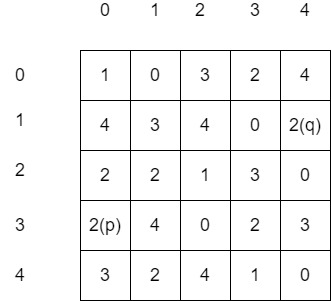
\includegraphics[width=0.5\linewidth]{input.jpg} \\ \\
V=\{4,2\} \\ 
The output returned is as follows : \\ \\
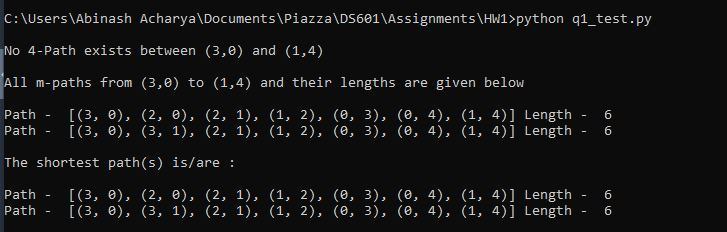
\includegraphics[width=\linewidth]{Q1_sample_output.JPG} \\ \\
As we can see, there are no 4-paths between p(3,0) and q(1,4) \\ 
There are 2 m-paths between p(3,0) and q(1,4). \\ 
Both are of same length i.e. 6. \\ 
So, both of them are listed as shortest m-paths. \\ 
These 2 m-paths have been shown in the figure below \\ \\
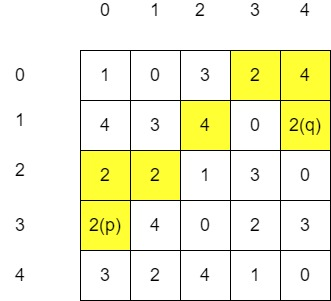
\includegraphics[width=0.5\linewidth]{m-path1.jpg} \\ \\
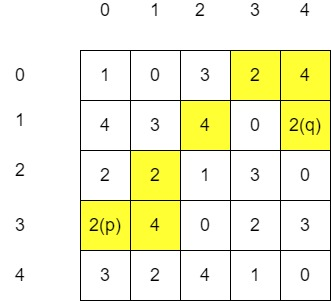
\includegraphics[width=0.5\linewidth]{m-path2.jpg} \\ \\
\section{Q2 Rectangle Creation}
The python file corresponding to this question is Q2.py. The user can specify the different parameters to generate different digital images as explained in the ReadME file. \\
The description of the main function is as follows:\\
create\_rectangles(M, N, border, n, w1, w2, alpha, orientation, vf, vb).
The various parameters are defined below:
\begin{itemize}
    \item (M,N): Specify the size of the image, i.e., the image is of size MxN.
    \item Border: It specifies the thickness of the black border around the image.
    \item n: The number of non-overlapping rectangles.
    \item (w1,w2): Specify the uniform distribution of widths of rectangles. 
    \item alpha: The ratio of height to width of the rectangles.
    \item orientation: The orientation of the image (Two possible orientations).
    \item vf: An array specifying the uniform distribution of all intensity values of foreground. Default = [0] (black).
    \item vb: An array specifying the uniform distribution of all intensity values of background. Default = [255] (white).
\end{itemize}
To handle cases where we are not able to find n non overlapping rectangles in the specified size MxN after $2*n$ iterations, we increase the size of image to 2Mx2N as suggested in the question.\\
Some examples of outputs of our function for different parameters specified by user are as follows:\\
M=400, N=400, border=4, n=25, alpha=2, w1=5, w2=20, vf=[0],vb =[255]\\
\begin{center}
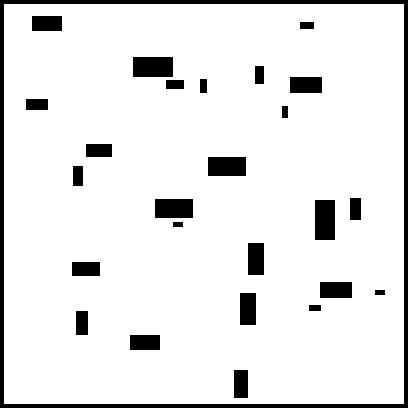
\includegraphics[scale=0.5]{rectangle1.jpg}
\end{center}
M=400, N=400, border=10, n=20, alpha=2, w1=5, w2=20, vf=[0, 1], vb=[129, 10, 255].\\
\begin{center}
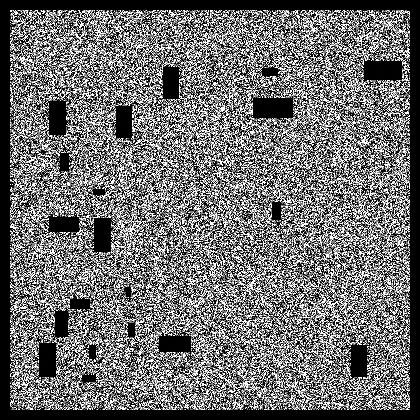
\includegraphics[scale=0.5]{rectangle.jpg}
\end{center}
We observe the above image because vf is randomly selected from [0,1] and vb from [129,10,255]. Another observation is that the border thickness has increased as we have specified it to be 10.
\end{document}
